\chapter{The ILD detector concept}
%\writer{Ties Behnke, Kiyotomo Kawagoe, Claude Vallee}{}


\section{The overall ILD concept}

The overall ILD concept has been kept unchanged since the DBD~\cite{ild:bib:ILDDBD}. The detector global layout and the performance of the subdetectors are tightly linked to the accelerator characteristics and the physics requirements, as summarized in figure ~\ref{fig:ILD:specifications}. 

\begin{figure}[t!]
\centering
%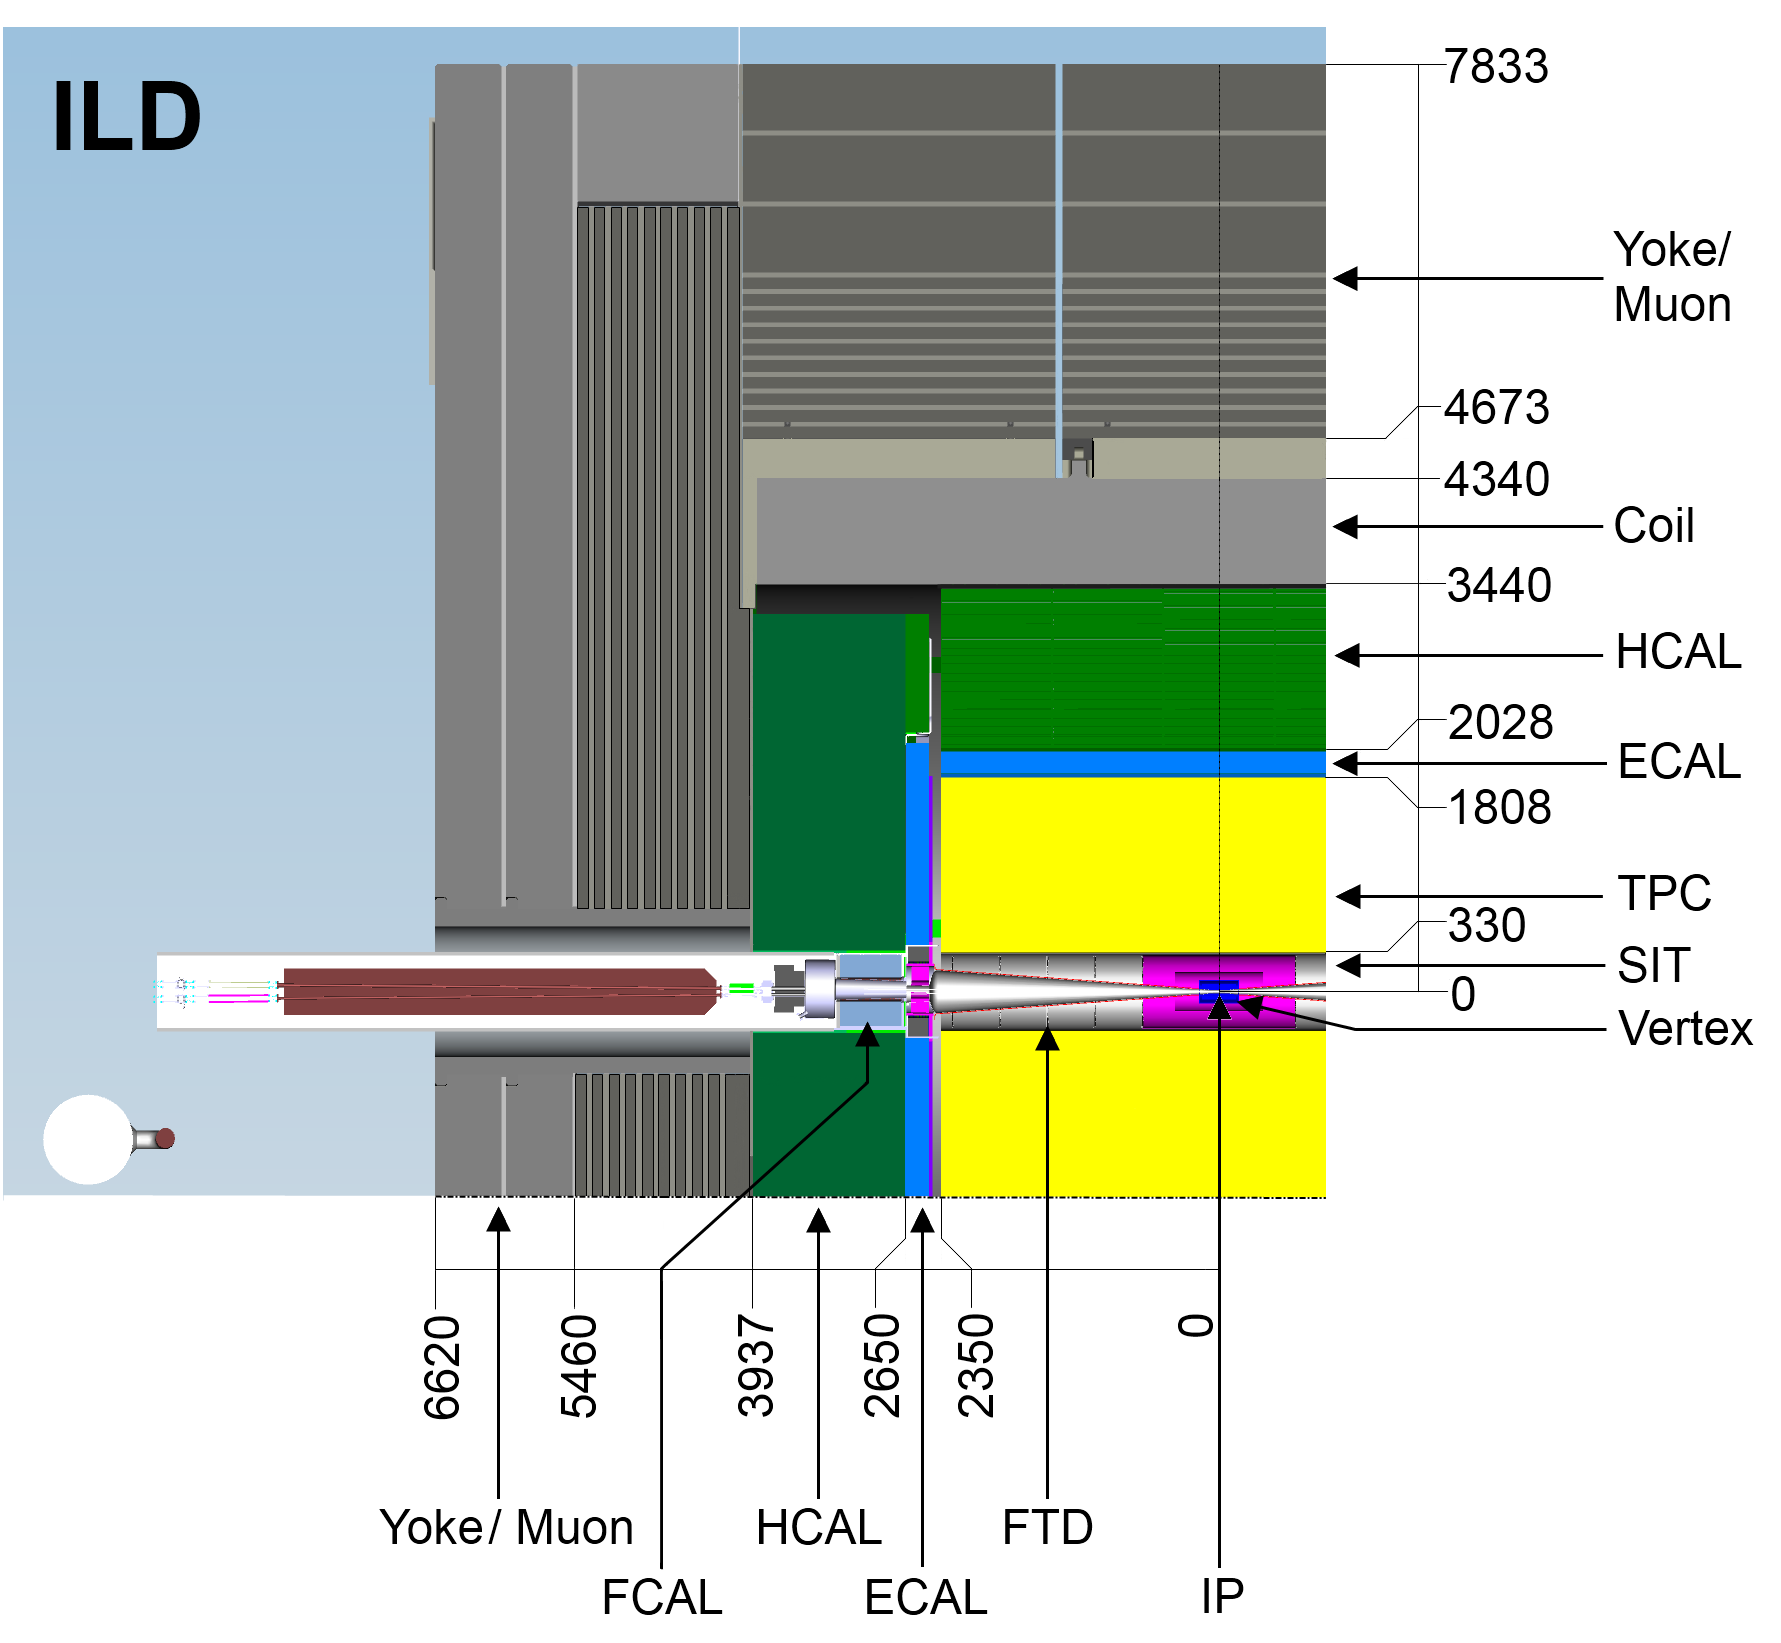
\includegraphics[width=0.8\hsize]{Detector/fig/ILD_quadrant_2.png}
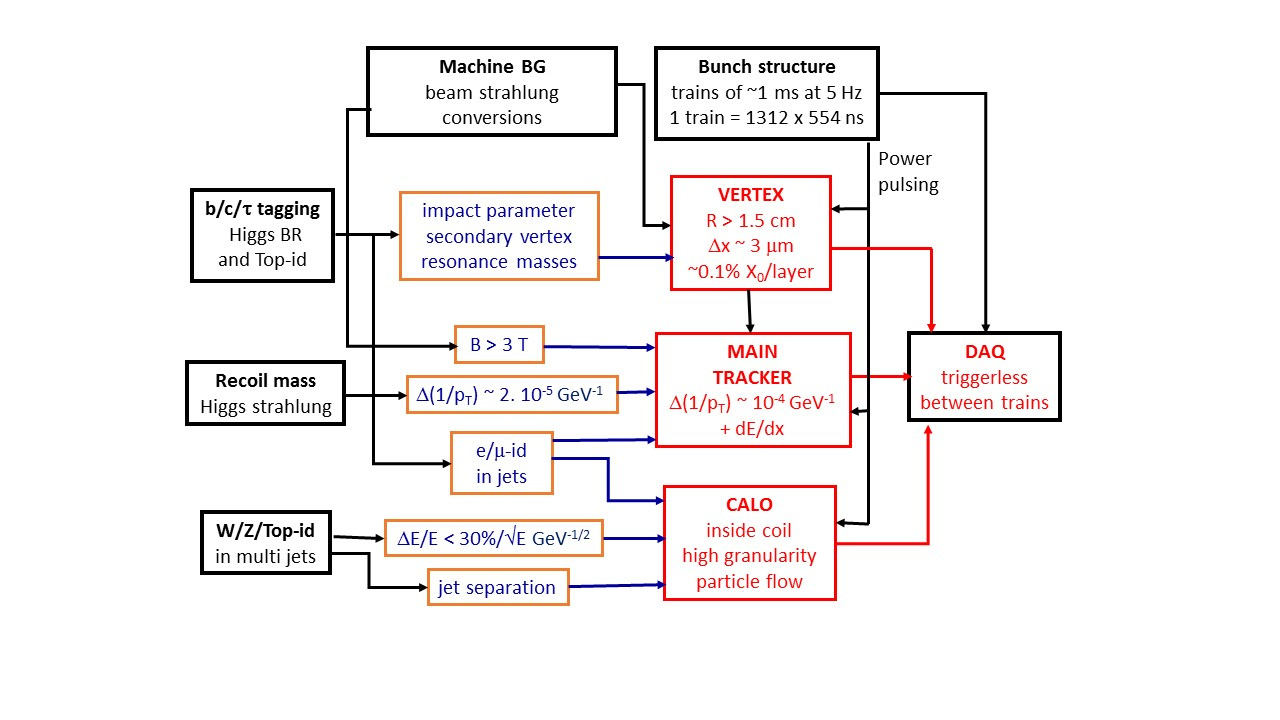
\includegraphics[width=1.2\hsize]{ILD/fig/ILD_specifications.jpg}
\caption{Interplay between ILC machine characteristics, physics requirements and detector specifications.}
\label{fig:ILD:specifications}
\end{figure}
	
The high beamstrahlung background at the collision point requires a magnetic field higher than 3T to maintain most of the conversion electron pairs confined within the beam pipe, and sets a minimum of $\approx$1.5 cm for the closest distance of approach of the vertex detector inner layer from the beamline. On the other hand the bunch structure of short trains separated by long idle periods sets rather relaxed conditions on the data acquisition, with the possibility to avoid a hardware trigger system. This in addition allows to power the front-end electronics only during active bunch trains (so-called "power-pulsing" mode), which minimizes the subdetector cooling requirements and associated material budgets.  

The subdetector specifications are tightly linked to the physics requirements from precision Higgs and electroweak physics. The dominant Higgs strahlung process, which at an $e^+e^-$ collider provides the unique opportunity to tag Higgs production independently of Higgs decay mode, requires a very high-precision momentum measurement of isolated particles from Z decays, which, even taking into account the high-precision inner silicon trackers, requires a high precision of the main tracker. The efficient tagging of quark and lepton flavours to disentangle Higgs couplings requires a very high precision and low-material vertex detector, as well as a high calorimeter granularity to identify leptons in jets. Similarly an efficient identification of W, Z and top hadronic decays in a crowded multijet environment needs a high jet energy resolution, twice better than currently realized at LHC, as well as an efficient spatial jet separation. ILD considers that the best concept to meet these requirements altogether is particle flow, where the charged and neutral particle contents of the jets are measured with the high performance trackers and the high granularity calorimeters, respectively. Within this scheme, an efficient match between the trackers and the calorimeters requires the calorimeters to be positioned inside the coil.     

%\textit{Detector performance aspects to be anticipated for higher energies}


\section{Optimising ILD}

The baseline ILD layout of the DBD~\cite{ild:bib:ILDDBD} had intentionally large dimensions in order to maximize the tracking performance and the particle flow capabilities of the calorimeters. The main cost drivers of the DBD detector were the electromagnetic calorimeter and the coil/yoke system. In the past years a re-optimization process of the detector global dimensions has been launched to identify an optimal point in the cost-performance space.

In a first step, a parametric study of the dependence of the cost and performance as function of the outer radius and length of the main tracker (a TPC in ILD) has been performed. The performance indicators were mainly based on Higgs precision observables and all subdetector costs were rescaled as function of their overall dimensions. The results of the study are summarized in figure ~\ref{fig:ILD:aspect_ratio}. This shows that targeting a given cost reduction maintains a higher performance when reducing the radius while keeping the overall length unchanged, instead of keeping the aspect ratio r/z unchanged.  

\begin{figure}[t!]
\centering
%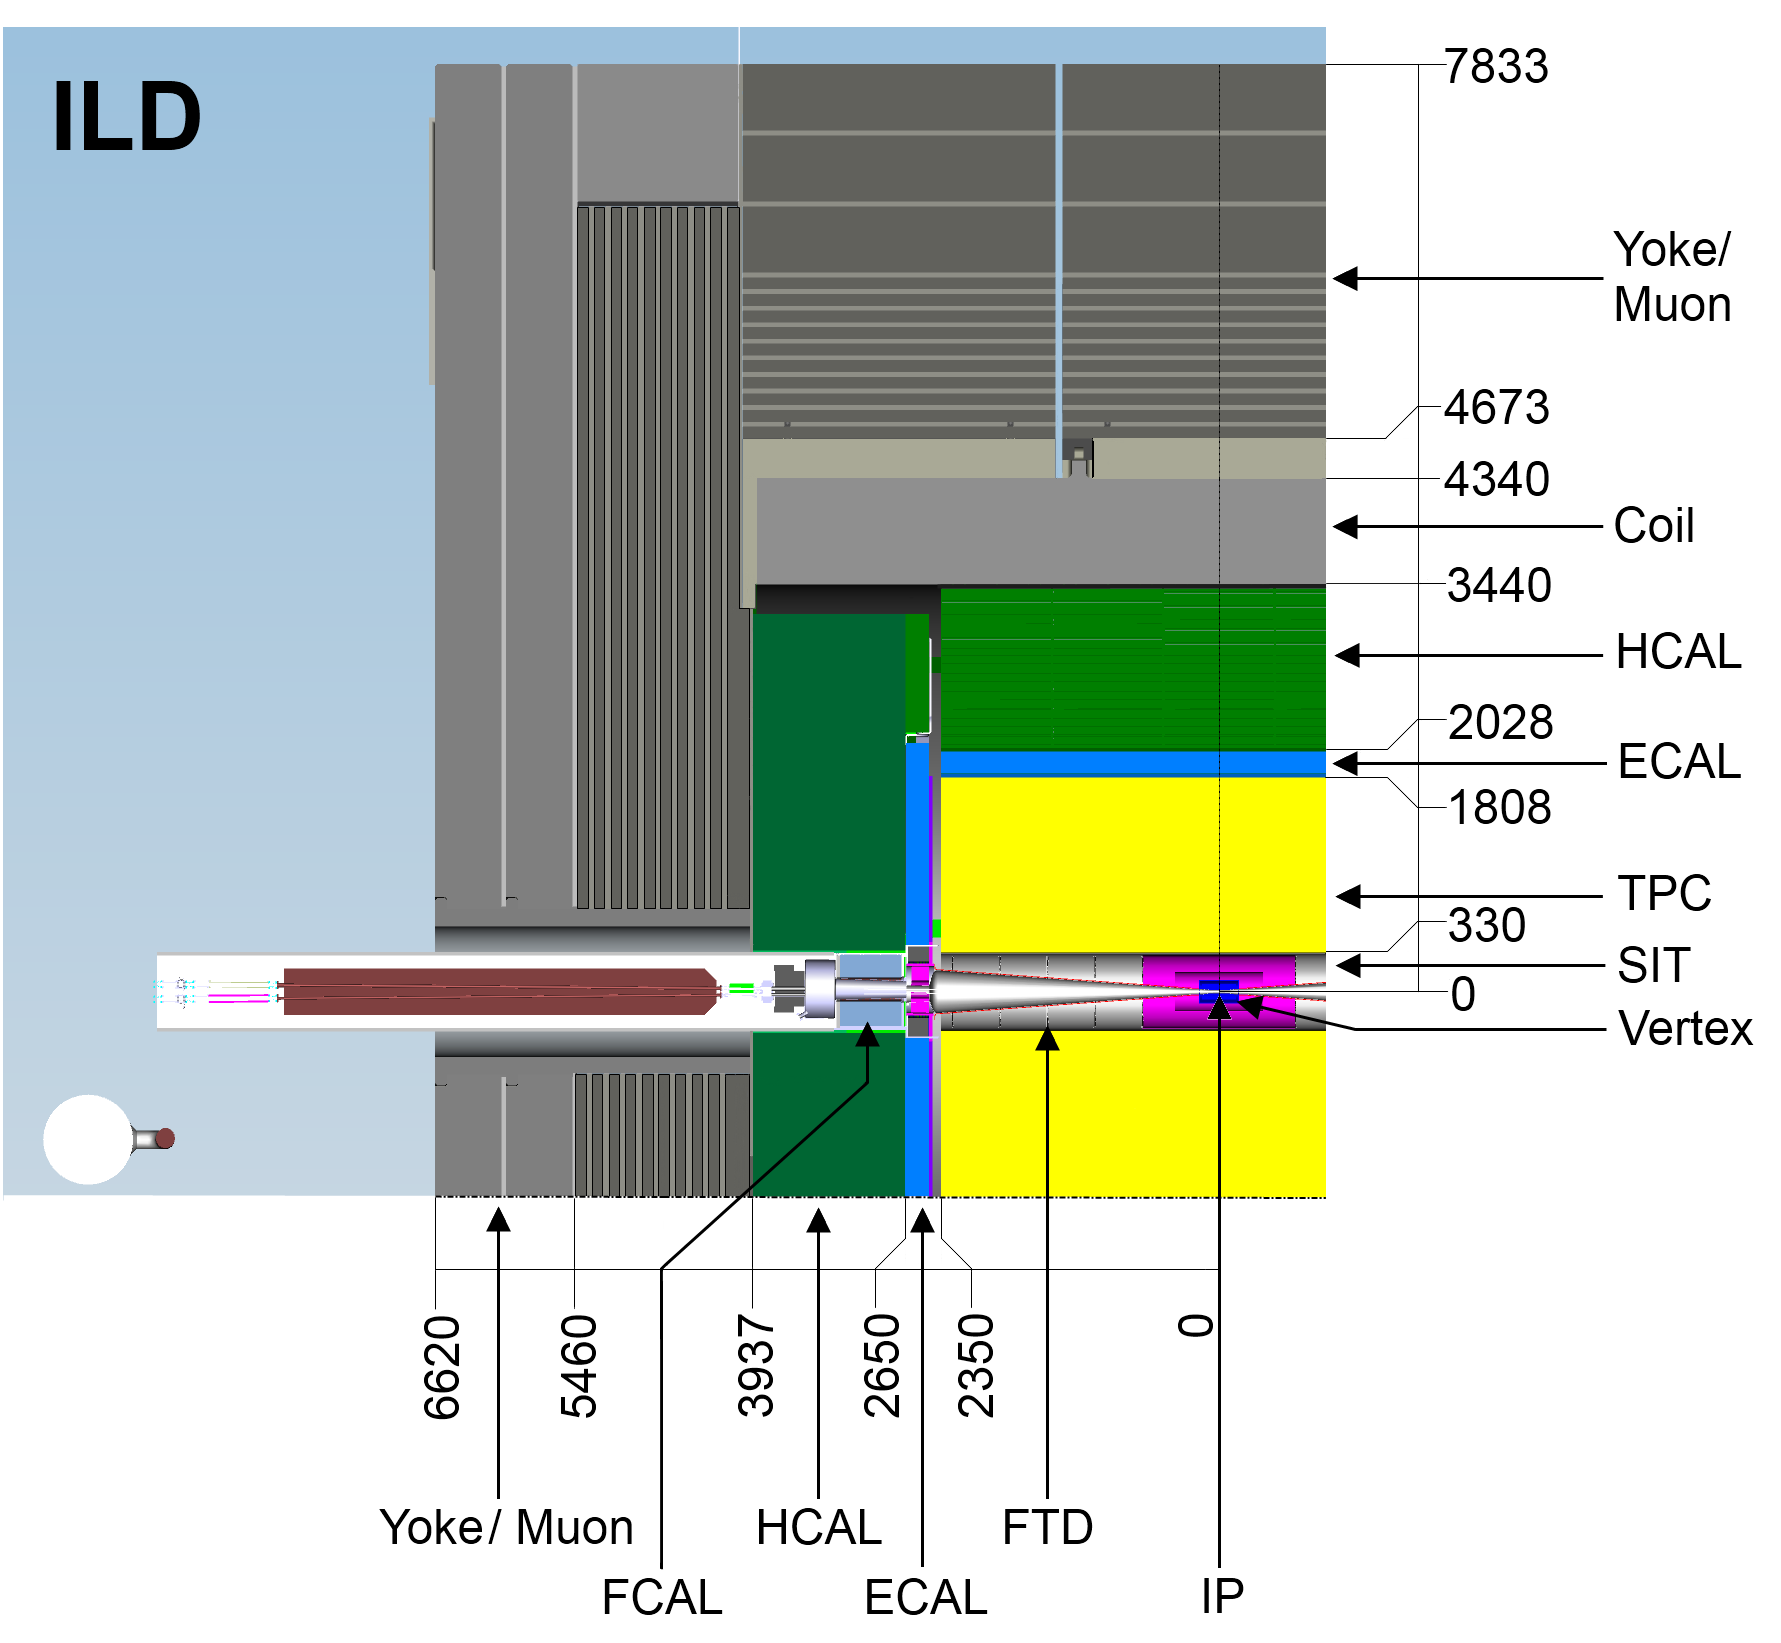
\includegraphics[width=0.8\hsize]{Detector/fig/ILD_quadrant_2.png}
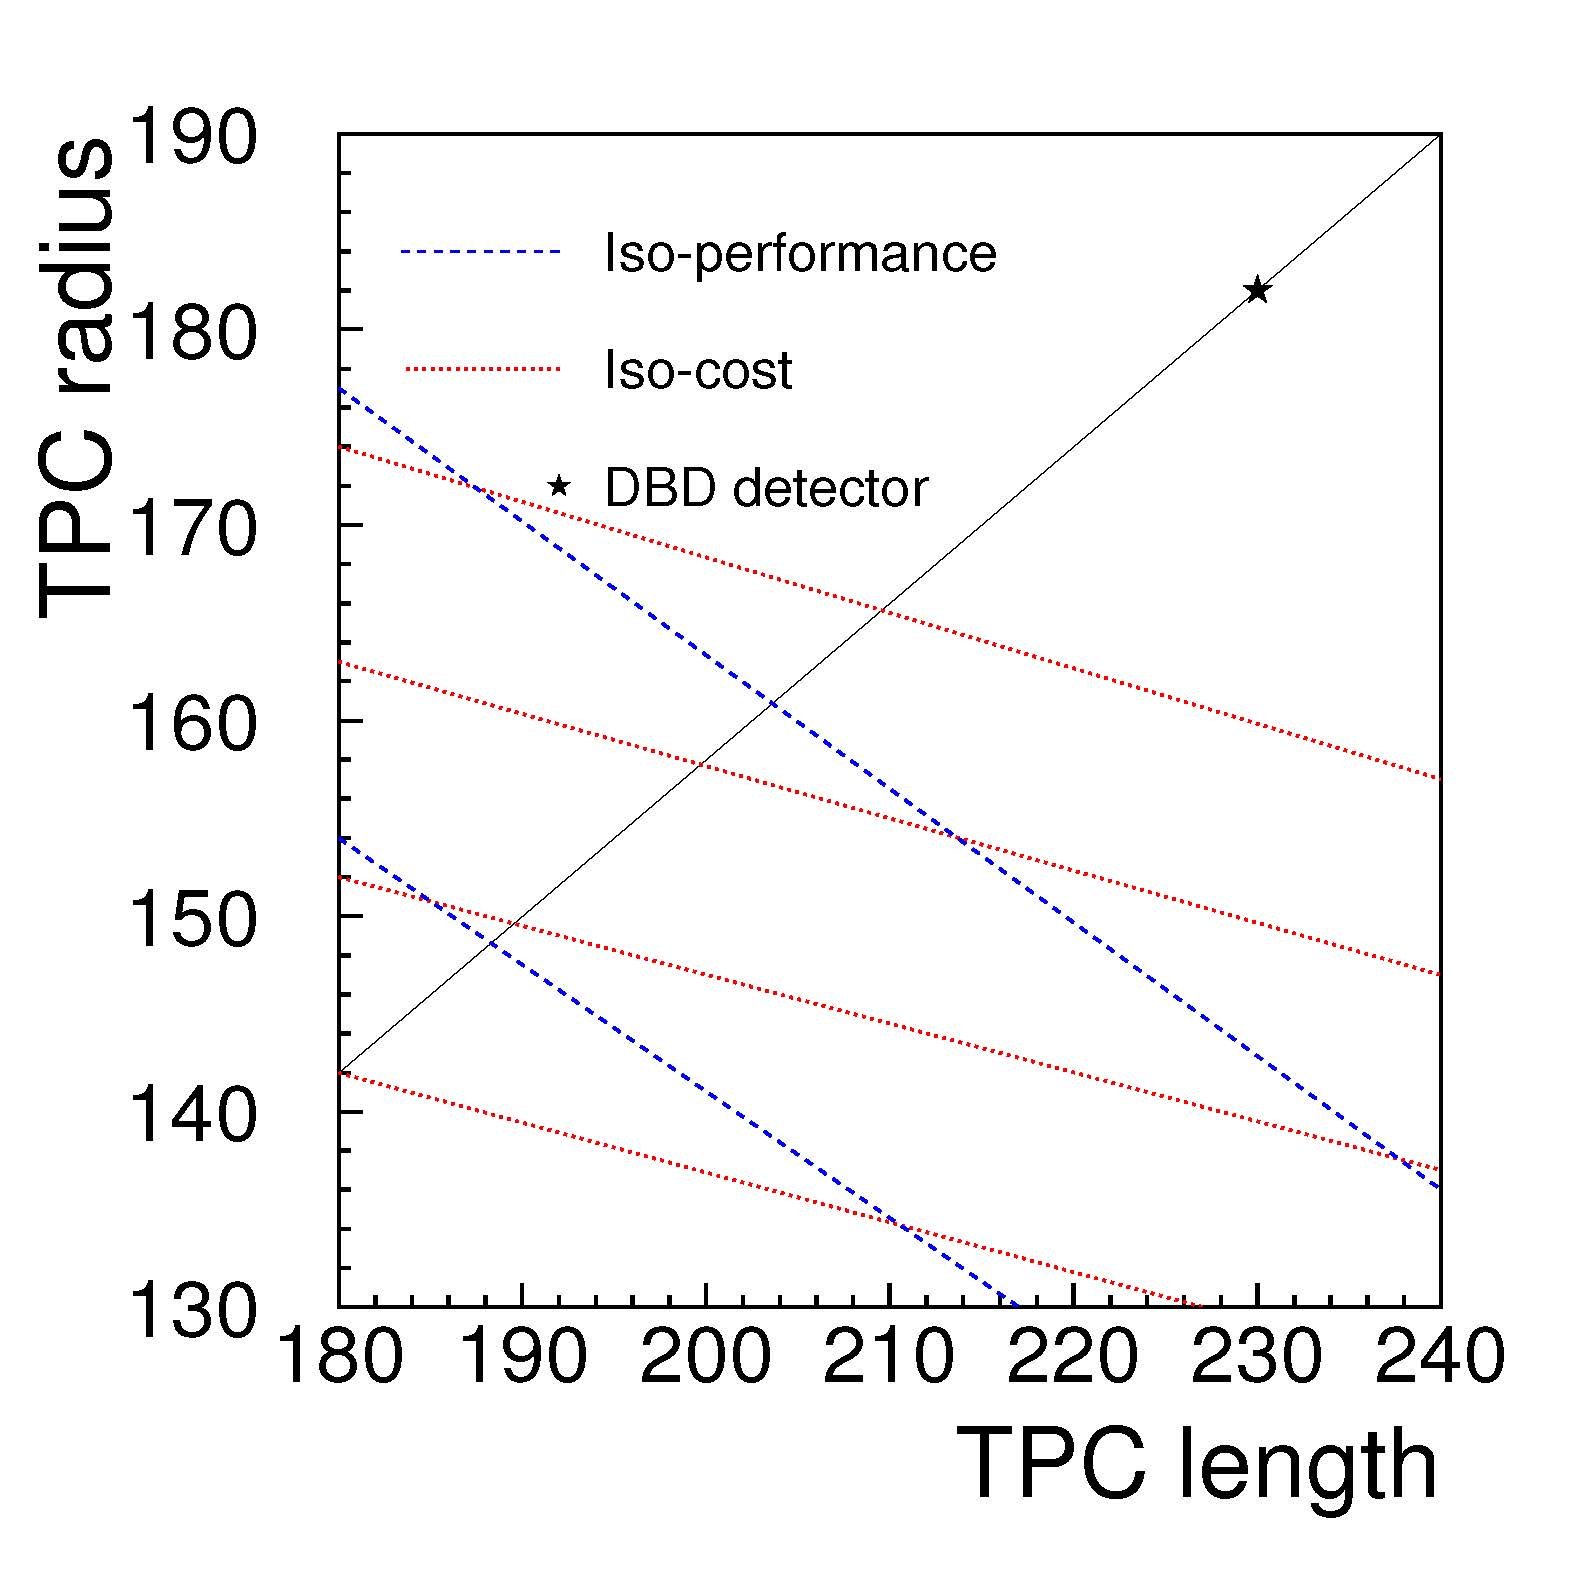
\includegraphics[width=0.6\hsize]{ILD/fig/aspect_ratio.jpg}
\caption{Iso-performance and iso-cost curves resulting from a parametric evaluation of the ILD detector in the tracker radius-length parameter space. The * corresponds to the DBD detector layout, close to the large IDR-L version. The diagonal indicates dimension changes at a constant r/z aspect ratio.}
\label{fig:ILD:aspect_ratio}
\end{figure}

Based on this study, detector models with different sizes were defined with the following guidelines:

\begin{itemize}
    
\item The number of detector models is limited to two to maintain simulations and analyses at a manageable level.

\item One of the models ("IDR-L") has dimensions similar to those of the DBD model, in order to have a well understood reference in the studies. The only changes compared to the DBD are associated to the collider parameter evolution (e.g. the new L* optics, see chapter 3), and to better understanding of the subdetector technology constraints.  

\item The second model ("IDR-S") has a reduced outer radius of the main tracker keeping its length unchanged. The smaller radius has to be far enough from the IDR-L radius to provide a significant level-arm for the comparison. The chosen value is equal to that of the new CLIC detector model CLICdp~\cite{Arominski:2018uuz}, half way of the further smaller radius of the SiD detector~\cite{ild:bib:ILDDBD}. With this choice IDR-S has similar outer tracker dimensions to CLICdp for both radius and length. This offers the possibility to compare the performance of the TPC option to the all-silicon option favored by CLICdp. 

\item All other components of IDR-S are similar to IDR-L. The inner tracking and very forward systems are identical. The calorimeter depths and cell sizes are also kept unchanged, and the number of cells reduced as function of the calorimeter radii. All external systems such as coil, yoke and endcaps have their radial dimensions reduced accordingly.

\item In order to compensate for the smaller tracking level arm the nominal magnetic field of IDR-S is increased from 3.5T to 4T.

\end{itemize}

The resulting IDR-L and IDR-S dimensions are summarized in figure ~\ref{fig:ILD:sizes}. Both models were used for detailed simulations of physics benchmark samples. The simulation framework is described in chapter 7. The detector and physics performance of both models are compared in chapter 8 and their costing estimated in chapter 9.

\begin{figure}[t!]
\centering
%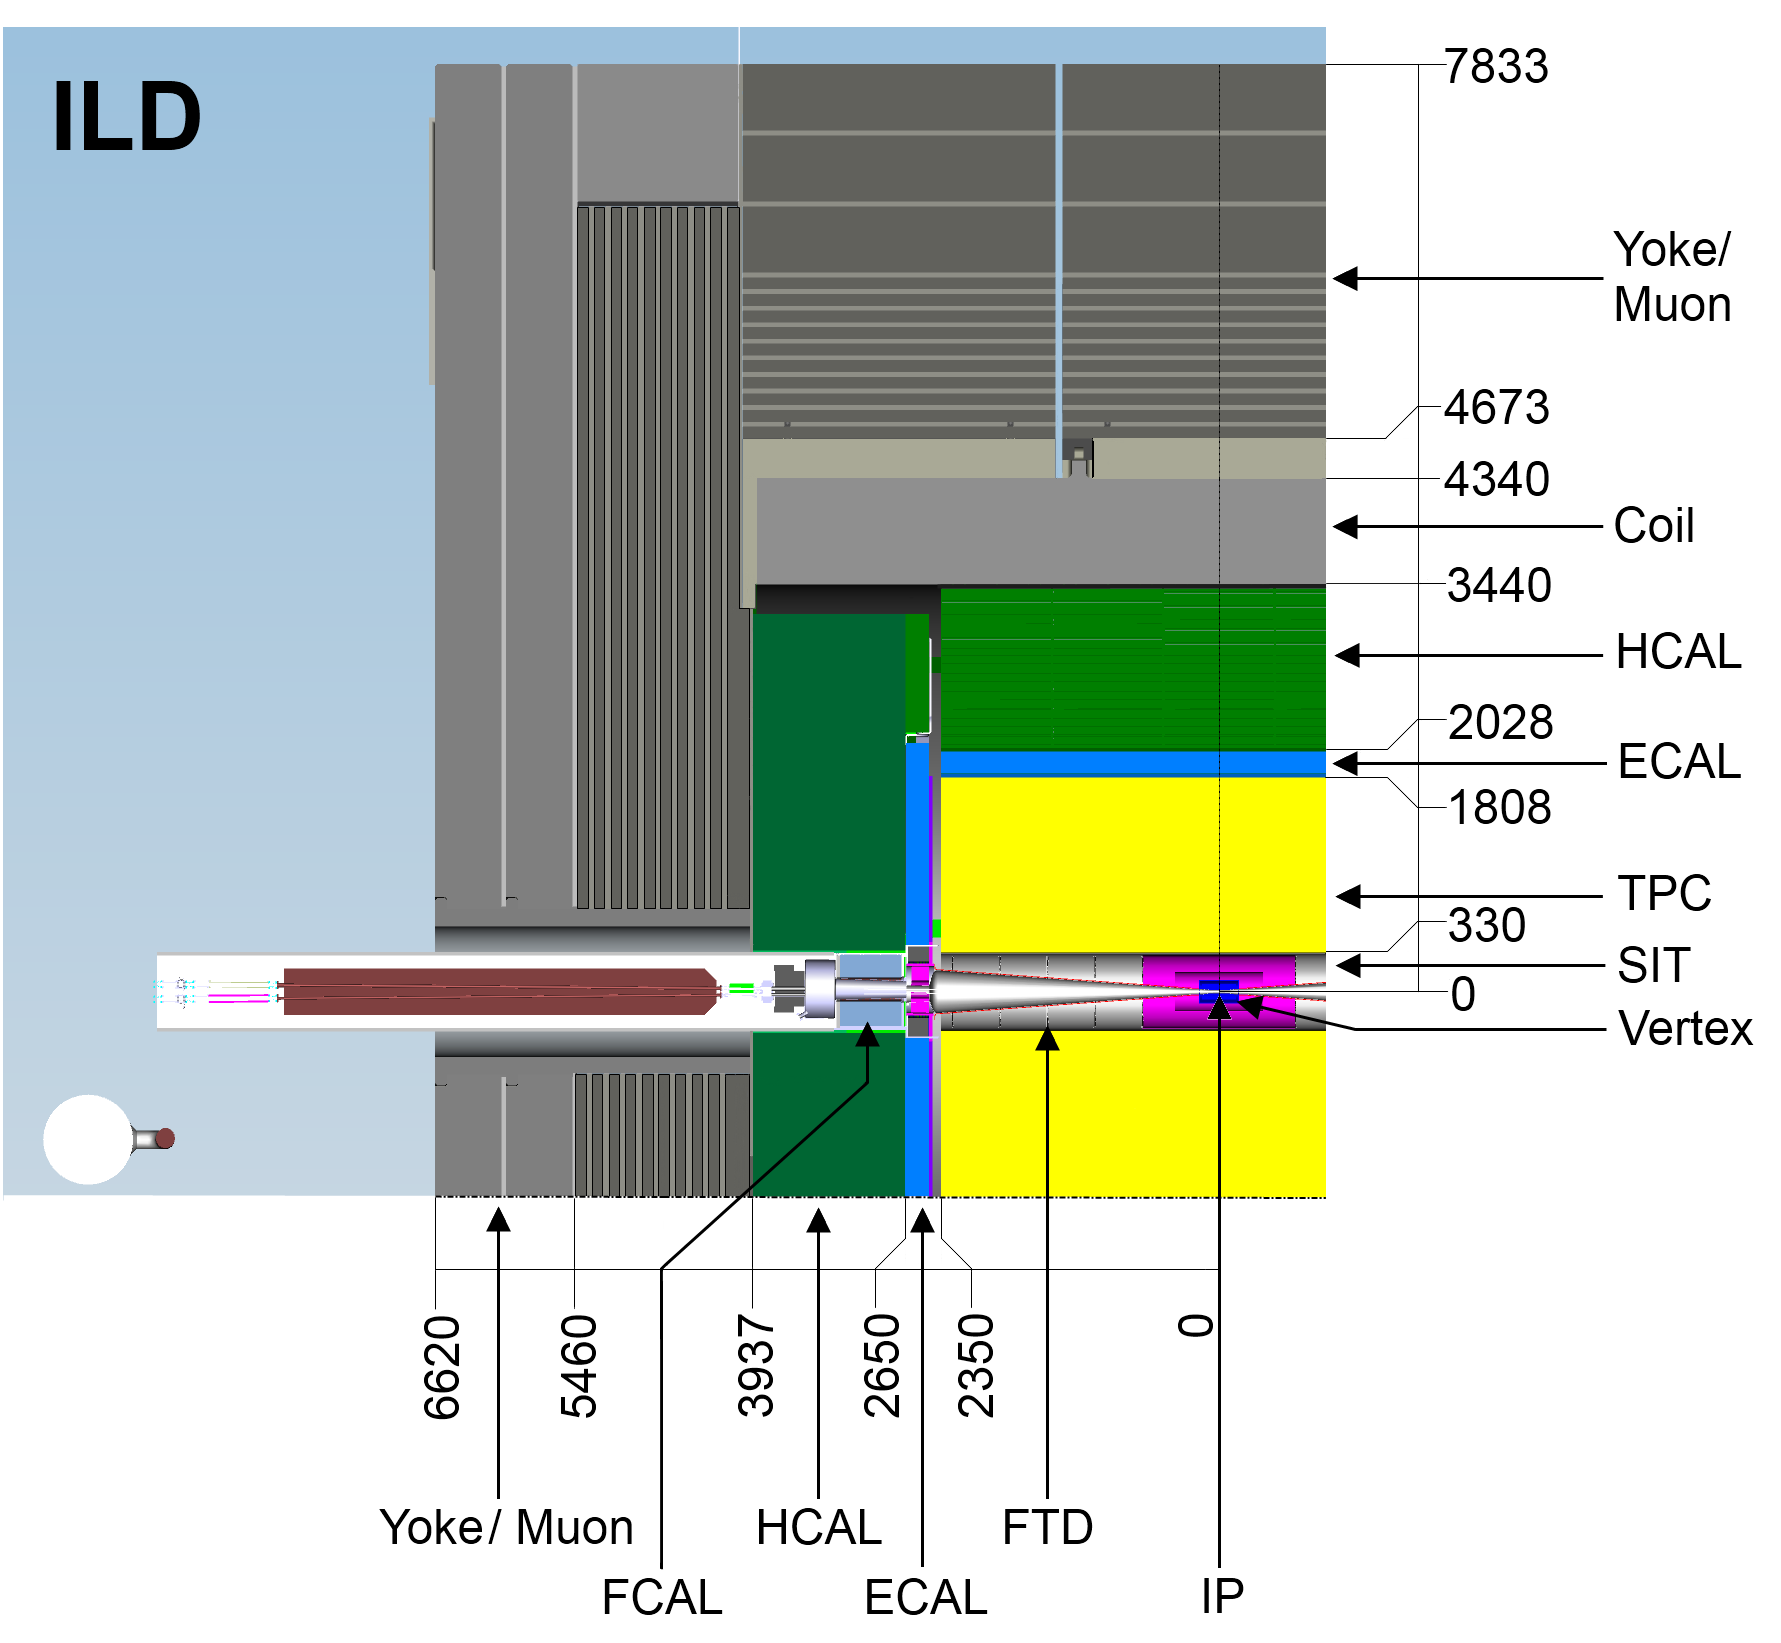
\includegraphics[width=0.8\hsize]{Detector/fig/ILD_quadrant_2.png}
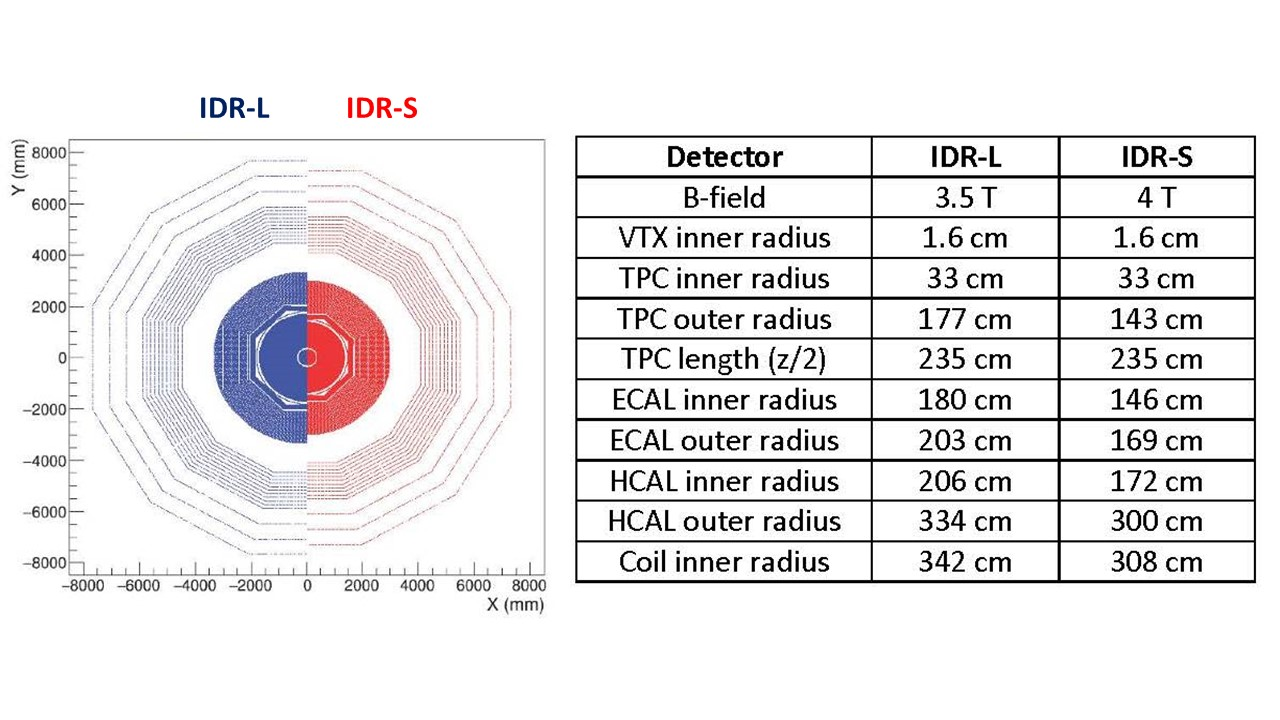
\includegraphics[width=1.0\hsize]{ILD/fig/ILD_small-large.jpg}
\caption{The large ("IDR-L") and small ("IDR-S") models used for the ILD optimization: R-$\phi$ view (left) and main subdetector dimensions (right).}
\label{fig:ILD:sizes}
\end{figure}
	